% Options for packages loaded elsewhere
\PassOptionsToPackage{unicode}{hyperref}
\PassOptionsToPackage{hyphens}{url}
\PassOptionsToPackage{dvipsnames,svgnames,x11names}{xcolor}
\documentclass[
  10pt,
  fontset=fandol]{ctexart}
\usepackage{xcolor}
\usepackage[margin=16mm]{geometry}
\usepackage{amsmath,amssymb}
\setcounter{secnumdepth}{-\maxdimen} % remove section numbering
\usepackage{iftex}
\ifPDFTeX
  \usepackage[T1]{fontenc}
  \usepackage[utf8]{inputenc}
  \usepackage{textcomp} % provide euro and other symbols
\else % if luatex or xetex
  \usepackage{unicode-math} % this also loads fontspec
  \defaultfontfeatures{Scale=MatchLowercase}
  \defaultfontfeatures[\rmfamily]{Ligatures=TeX,Scale=1}
\fi
\usepackage{lmodern}
\ifPDFTeX\else
  % xetex/luatex font selection
\fi
% Use upquote if available, for straight quotes in verbatim environments
\IfFileExists{upquote.sty}{\usepackage{upquote}}{}
\IfFileExists{microtype.sty}{% use microtype if available
  \usepackage[]{microtype}
  \UseMicrotypeSet[protrusion]{basicmath} % disable protrusion for tt fonts
}{}
\makeatletter
\@ifundefined{KOMAClassName}{% if non-KOMA class
  \IfFileExists{parskip.sty}{%
    \usepackage{parskip}
  }{% else
    \setlength{\parindent}{0pt}
    \setlength{\parskip}{6pt plus 2pt minus 1pt}}
}{% if KOMA class
  \KOMAoptions{parskip=half}}
\makeatother
\usepackage{graphicx}
\makeatletter
\newsavebox\pandoc@box
\newcommand*\pandocbounded[1]{% scales image to fit in text height/width
  \sbox\pandoc@box{#1}%
  \Gscale@div\@tempa{\textheight}{\dimexpr\ht\pandoc@box+\dp\pandoc@box\relax}%
  \Gscale@div\@tempb{\linewidth}{\wd\pandoc@box}%
  \ifdim\@tempb\p@<\@tempa\p@\let\@tempa\@tempb\fi% select the smaller of both
  \ifdim\@tempa\p@<\p@\scalebox{\@tempa}{\usebox\pandoc@box}%
  \else\usebox{\pandoc@box}%
  \fi%
}
% Set default figure placement to htbp
\def\fps@figure{htbp}
\makeatother
\setlength{\emergencystretch}{3em} % prevent overfull lines
\providecommand{\tightlist}{%
  \setlength{\itemsep}{0pt}\setlength{\parskip}{0pt}}
\usepackage{amsmath,amssymb,mathtools,needspace}
\xeCJKDeclareCharClass{CJK}{"2032,"0400->"04FF,"2160->"216B,"2460->"2473,"25A0,"25C7,"25CB,"25CF}
\IfFontExistsTF{Arial Unicode MS}{\xeCJKsetup{AutoFallBack=true}\setCJKfallbackfamilyfont{\CJKrmdefault}{Arial Unicode MS}}{}
\setcounter{secnumdepth}{0}
\setlength{\emergencystretch}{2em}
\allowdisplaybreaks
\usepackage{bookmark}
\IfFileExists{xurl.sty}{\usepackage{xurl}}{} % add URL line breaks if available
\urlstyle{same}
\hypersetup{
  pdftitle={试射法},
  colorlinks=true,
  linkcolor={Maroon},
  filecolor={Maroon},
  citecolor={Blue},
  urlcolor={Blue},
  pdfcreator={LaTeX via pandoc}}

\title{试射法}
\author{}
\date{}

\begin{document}
\maketitle

\subsubsection{5.7.1 试射法}\label{ux8bd5ux5c04ux6cd5}

可以用所谓``试射法''来求解边值问题（5.7.1）、（5.7.3）。这种方法的基本思想是设法将边值问题转化为初值问题来求解，即依据边界条件（5.7.3）寻求与它等价的初始条件（5.7.2），也就是说，反复调整初始时刻的斜率值 \(y'(a)=m\)，使初值问题（5.7.1）、（5.7.2）的积分曲线 \(y=y(x)\) 能``命中''\(y(b)=\beta\)（见图 5.5）。

试射法的计算过程很简单。设凭经验能够提供 \(m\) 的两个预测值 \(m_1,m_2\)，分别按这两个斜率值``试射''------求解相应的初值问题（5.7.1）、（5.7.2），从而获得 \(y(b)\) 的两个结果 \(\beta_1,\beta_2\)。如果 \(\beta_1\) 与 \(\beta_2\) 均不满足预定的精度，就用线性插值方法校正 \(m_1,m_2\) 得新的斜率值

\[
m_3=m_1+\frac{m_2-m_1}{\beta_2-\beta_1}(\beta-\beta_1),
\]

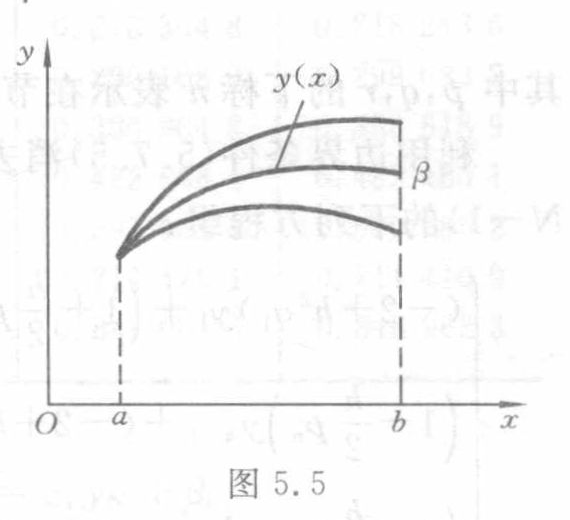
\includegraphics[width=0.85\linewidth,height=\textheight,keepaspectratio,alt={图 5.5（原图）试射法示意}]{../assets/ch05b/figure-5-5.png}

图 5.5（原图）符号与图意：坐标轴 \(x,y\)，原点 \(O\)，横轴端点 \(a,b\)，目标右端值 \(\beta\)，积分曲线标记 \(y(x)\)。三条曲线从 \(x=a\) 的同一左端点出发，在 \(x=b\) 处到达不同高度；\(y(x)\) 指向达到目标 \(\beta\) 的中间曲线。端点位置以竖虚线标出；图中未给出具体函数或数值。

然后再按斜率值 \(m_3\) 试射，求解相应的初值问题（5.7.1）、（5.7.2），又得新的结果 \(y(b)=\beta_3\)。继续这一过程，直到计算结果 \(y(b)\) 与 \(\beta\) 相当符合为止。

上述试射法过分依赖于经验，局限性大。下面介绍求解边值问题的差分方法。

\end{document}
